\documentclass[12pt,letterpaper]{article}
\usepackage[margin=1in]{geometry}

\usepackage[utf8]{inputenc} % OJO!!!  => MANTENER ESTA LINEA PARA FACIL CONVERSION A WORD EN EL FUTURO ...
% \usepackage[spanish]{babel}
\usepackage{graphicx} 
\usepackage{array}
\usepackage{tabularx}
\usepackage{amssymb, amsmath}

% Paquetes extras ... 
\usepackage{subfigure}
\usepackage{color}
\definecolor{mygreen}{RGB}{28,172,0} % color values Red, Green, Blue
\definecolor{mylilas}{RGB}{170,55,241}

\usepackage{hyperref}
\usepackage{enumitem}

\usepackage{amsmath,amsfonts,amssymb,amsthm,cancel,icomma,nicefrac,mathrsfs,
            eurosym,verbatim,environ,ifthen,ifdraft,pdfpages,float,booktabs}
\allowdisplaybreaks[1] 

\usepackage{color}
\definecolor{lstgrey}{rgb}{0.95,0.95,0.95}
\usepackage{listings}
\lstset{language=Matlab,
       backgroundcolor=\color{lstgrey},
       frame=single,
       basicstyle=\footnotesize\ttfamily,
       captionpos=b,
       tabsize=2,
  }

\lstset{language=Matlab,%
  %basicstyle=\color{red},
  breaklines=true,%
  morekeywords={matlab2tikz},
  keywordstyle=\color{blue},%
  morekeywords=[2]{1}, keywordstyle=[2]{\color{black}},
  identifierstyle=\color{black},%
  stringstyle=\color{mylilas},
  commentstyle=\color{mygreen},%
  showstringspaces=false,%without this there will be a symbol in the places where there is a space
  numbers=left,%
  numberstyle={\tiny \color{black}},% size of the numbers
  numbersep=9pt, % this defines how far the numbers are from the text
  emph=[1]{for,end,break},emphstyle=[1]\color{red}, %some words to emphasise
  %emph=[2]{word1,word2}, emphstyle=[2]{style},    
}

\title{Asignment 5}
\author{Jose Eduardo Laruta Espejo \\ Facultad de Ingeniería - Universidad Mayor de San Andrés}
\begin{document}
\maketitle
\section{Problem 1}

The autocorrelation matrix $R$ is given by:
\begin{equation*}
  R = E[\underline{u_n} \underline{u_n}^{T}]
\end{equation*}
and the channel is $h = [h_0 \ h_1]^T$. For N = 32 and because $\underline{h}$ has only 2 elements in it, 
we can define our $R$ matrix as follows:
\begin{align}
  R &= \begin{bmatrix}
    r(0)    & r(1)  & 0       & \cdots  & 0       & 0       \\
    r(1)    & r(0)  & r(1)    & 0       & \cdots  & 0       \\
    \vdots  &       &         &         &         & \vdots \\
    0       & \cdots& 0       & r(1)    & r(0)    & r(1)    \\
    0       & 0     & \cdots  & 0       & r(1)    & r(0)
  \end{bmatrix} \\
  r(0) &= \sigma_\eta^2 + \sigma_b^2 (h_0^2 + h_1^2) \\
  r(1) &= \sigma_b (h_0 h_1)\label{eq:r1}
\end{align}

the following MATLAB code was used for building the R matrix and obtain the ratio of eigenvalues:

\lstinputlisting[label={lst:code1}, caption={Code for Problem 1}]{../matlab/rmatrix.m}

for $\underline{h} = [1 \  1]^T$ the ratio between the maximum eigenvalue and the minimum eigenvalue is:
$$ratio = \frac{\lambda_{max}}{\lambda_{min}} = 396.9652$$


if we make $h_1 = 0$ (from Eq. \ref{eq:r1}) we have $r(1)$ = 0, then $R$ is a diagonal matrix with $r(0)$ 
all over its diagonal, then, all the eigenvalues are the same, hence, the ratio would be 1. Running the code 
we can see this occurs in MATLAB as well:
$$ratio = \frac{\lambda_{max}}{\lambda_{min}} = 1$$


\section{Problem 2}

% \begin{figure}[!h] 
%   \centering
%   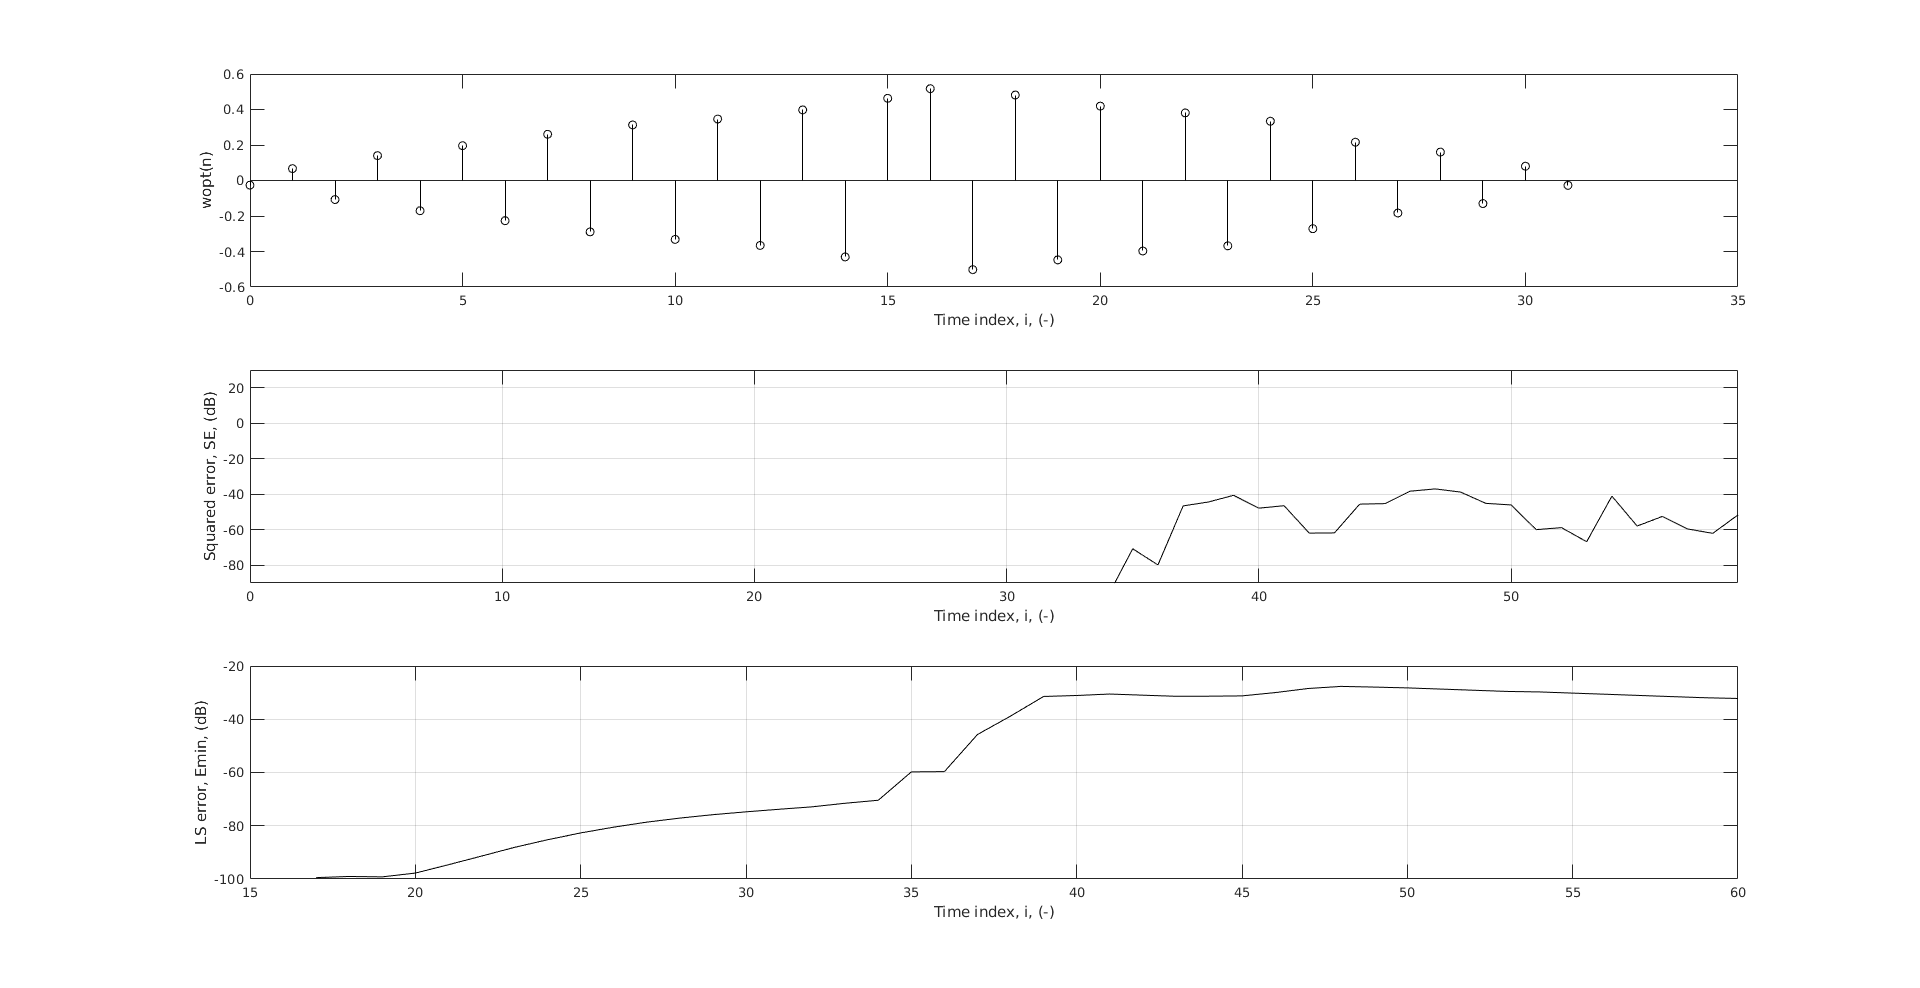
\includegraphics[width=1\textwidth]{../matlab/img/plots.png}
%   \caption{plots for RLS example ($\lambda = 0.95$)}
%   \label{fig:res}
% \end{figure}
\newpage
\section{Problem 3}


\end{document}